\subsubsection{依据观测更新搜索状态并计算任务总耗时}\label{sec:q3-1}

记第 \(t\) 次真实动作后的信息状态为

\begin{equation}\label{eq:q3-1}
S_t=\left(x_t,f_t,T_t,\mathcal D_t,\mathcal K_t,
\{\widehat C_f,\mathcal O_f^+,\mathcal O_f^-\},P_t,F_t\right).
\end{equation}

其中 \(x_t,f_t\) 为位置和当前测向频道，\(T_t\) 为累计虚拟时间；
\(\mathcal D_t\)、\(\mathcal K_t\) 分别记录已发现、已成功清除的频道；
\(\mathcal O_f^+\)、\(\mathcal O_f^-\) 为同频道正、负反馈；
\(P_t\) 为已完成的发现站集合，\(F_t\) 为未来覆盖站。
源位置、实际源数和各源接收半径不进入决策状态。

总虚拟时间按实际动作计为

\begin{equation}\label{eq:q3-2}
T=\frac{L}{v}+N_{\rm switch}+5N_{\rm measure}
+3N_{\rm clear}+2K,\qquad v=5.
\end{equation}

这里 \(N_{\rm clear}\) 包含成功与失败的光学尝试，\(K\) 为成功次数；
清除不改变测向频道。
优化目标是在全清约束下减小 \(T\)。
算法自身的计算时间另外记录，不能与机器人虚拟时间混合。

正示向反馈按第二问更新区域。
对于已确认存在的全向源，若在 \(x^+\) 有信号、在 \(x^-\) 无信号，由同一接收半径固定可得

\begin{equation}\label{eq:q3-3}
\|p-x^+\|\le R_f<\|p-x^-\|
\Longrightarrow
(x^--x^+)^Tp\le\frac{\|x^-\|^2-\|x^+\|^2}{2}.
\end{equation}

右侧取闭半平面作为严格不等式的保守放宽。
将新观测与所有异类历史观测配对裁剪，使无信号反馈也能够缩小区域。
尚未出现正观测时只保存负点；
不将一次无信号直接解释为频道无源。
该距离关系依赖全向辐射，不能直接用于第四问。

\subsubsection{布置七个检测点覆盖目标区域并调整后续检测位置}\label{sec:q3-2}

先在原点扫描20个频道，再以原点与半径 \(a=1150\) m圆周上的6个等角站构成初始覆盖：

\begin{equation}\label{eq:q3-4}
P_0=\{(0,0)\}\cup
\{a(\cos(k\pi/3),\sin(k\pi/3)):k=0,\ldots,5\}.
\end{equation}

对任意 \(p\in\Omega\)，若 \(\|p\|\le1000\)，则原点必能接收；
否则记 \(r=\|p\|\in[1000,1800]\)，存在一个环上站与其极角相差不超过 \(30^\circ\)，于是

\begin{equation}\label{eq:q3-5}
\|p-x_k\|^2\le r^2+a^2-\sqrt3ar.
\end{equation}

右侧关于 \(r\) 为凸函数，在该区间的最大值取于端点。
代入 \(a=1150\)，两端均小于 \(1000^2\)，故七个站覆盖所有可能源位置。
只要每个仍未知频道在覆盖站完成实际扫描，就不会遗漏全向源。
已清除频道无须再测；
已持有可靠清除位置的已知频道也可省略后续扫描。

固定覆盖站提供完整性，却可能迫使机器人在已知源附近绕行。
因此允许移动一个尚未执行的站，同时保留全覆盖。
设待改站为 \(x_i\)，\(G_i\) 包含已执行站与其余未来站，取 \(r_s=1000-10^{-5}\) m，尚需由此站负责的区域为

\begin{equation}\label{eq:q3-6}
E_i=\Omega\setminus\bigcup_{x\in G_i}B(x,r_s),
\qquad Q_i^{\rm cover}=\bigcap_{p\in E_i}B(p,r_s).
\end{equation}

新站 \(y\in Q_i^{\rm cover}\) 即可保持覆盖；
该集合是圆盘的交，因而为凸集。
以旧站为起点，朝当前位置、邻近已知源代表点及相关投影点试探，沿线段二分寻找可行位置，再比较更新后的路线费用。
每轮至多改变一个站，旧位置始终保留为可行备选。

实际覆盖核验计算

\begin{equation}\label{eq:q3-7}
\Gamma(P)=\max_{p\in\Omega}\min_{x\in P}\|p-x\|,
\end{equation}

要求 \(\Gamma(P)\le r_s\)。
计算检查最近站Voronoi结构的内部顶点、圆周交点与圆弧极值，不以只检查场地圆周代替全域覆盖。
未来站的可行性属于计划约束；
只有实际扫描完成后，才能计入发现证据。

\begin{figure}[!htbp]
\centering
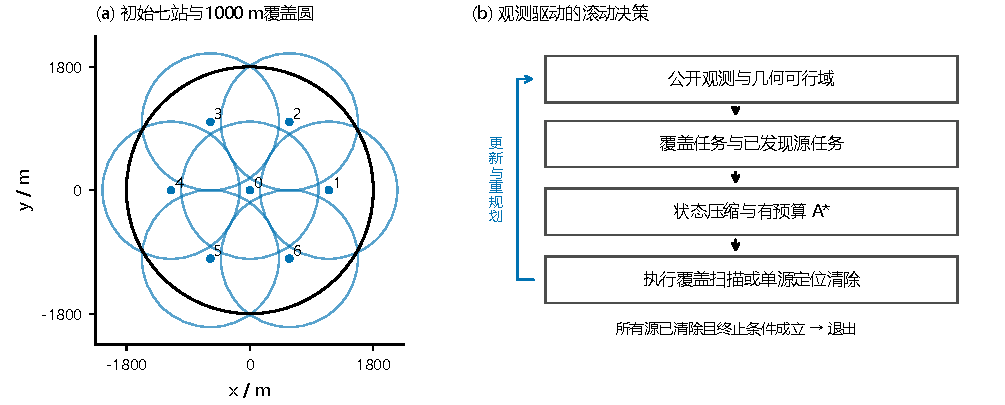
\includegraphics[width=\linewidth,height=\textheight,keepaspectratio,alt={初始发现覆盖与滚动决策框架。七个1000 m接收保证圆覆盖半径1800 m场地；未来站移动后仍需重新通过全域覆盖核验。}]{figures/fig02_framework.pdf}
\caption{初始发现覆盖与滚动决策框架。七个1000 m接收保证圆覆盖半径1800 m场地；未来站移动后仍需重新通过全域覆盖核验。}
\label{fig:q23-2}
\end{figure}

\subsubsection{利用状态压缩与A*搜索安排当前任务的执行顺序}\label{sec:q3-3}

每完成一次覆盖扫描或一个源的处理，构造两类当前任务：尚未执行的覆盖站，以及已发现但未清除的源。
源任务以近场点或可行域包围圆心作为代表位置 \(y_i\)。
这些位置来自观测估计，实际定位仍由第二问模块完成，故源任务的代表点与最终清除点可以不同。

在本轮规划内冻结任务集合、位置和服务费用。
设有 \(n\) 个任务，\(M\) 为已完成任务集合，程序以位掩码编码，\(j\) 为最后任务；
起始状态 \((\varnothing,-1)\) 对应当前位置，约定 \(y_{-1}=x_t\)。
借鉴子集动态规划\cite{held1962}，将不同访问顺序压缩成相同的 \((M,j)\)，定义 \(g(M,j)\) 为到达该状态的最小前缀费用。
转移为

\begin{equation}\label{eq:q3-8}
g(M\cup\{i\},i)=\min_j\left[g(M,j)+\Delta(M,j,i)\right],
\end{equation}

\begin{equation}\label{eq:q3-9}
\Delta(M,j,i)=\frac{\|y_j-y_i\|}{v}+s_i
+q\,\mathbf1_{\{i\text{为覆盖任务}\}}\,|\mathcal S\setminus M|.
\end{equation}

其中 \(\mathcal S\) 是本轮源任务集合，\(s_i\) 对源任务取5 s，对覆盖任务取 \(6b\) s，\(b=\max\{0,20-|\mathcal K_t|-|\mathcal S|\}\)。
最后一项用于表示覆盖访问时尚未处理源的附加扫描费用。
第一版选定配置取 \(q=0\)，使当前排序主要由旅行距离决定；
实际测量与换频仍按式\eqref{eq:q3-2}完整计费。
冻结服务费只用于比较候选路线，不替代实际时间账。

若两个前缀到达同一 \((M,j)\)，其后续任务、起点和费用函数完全相同，较贵前缀不会产生更优完整路线，因而可以删除。
这一支配关系将排列枚举压缩为至多 \(O(n2^n)\) 个状态、\(O(n^22^n)\) 条转移。
这里压缩的是一次规划中的任务顺序，并未把具有不同观测历史的真实世界状态强行合并。

采用A*启发式图搜索\cite{hart1968}，为优先探索有希望的前缀，对未完成任务集 \(U\) 构造下界

\begin{equation}\label{eq:q3-10}
h(M,j)=\frac{\min_{i\in U}\|y_j-y_i\|+\operatorname{MST}(U)}{v}
+\sum_{i\in U}s_i.
\end{equation}

其中 \(U=\varnothing\) 时取零。
任何完整后缀都必须先接入 \(U\)，再连通其中全部任务，其旅行距离不小于最近接入边加最小生成树；
省略非负附加扫描费不会抬高下界。

算法先由最近邻和开路2-opt得到完整可行路线，费用记为 \(U_t\)；
再按 \(g+h\) 从小到大展开，结合状态支配和 \(g+h\ge U_t\) 上界剪枝。
发现更短完整路线时更新 \(U_t\)。
预算耗尽则返回当前可行路线及前沿下界 \(L_t\)；
搜索闭合时两界相等。
实现保留 \(10^{-9}\) s比较容差，并允许改进状态重新入队。

当前任务至多22个；
选定配置每次搜索至多展开100个状态，整局总展开上限为60000。
只执行返回顺序的第一个任务，随后重新构造问题。
\(U_t-L_t\) 衡量本轮冻结代理模型的求解缺口；
未来新源、反馈分支和定位绕路未被完整枚举，因此它不是第三问在线最优策略的差距。

\subsubsection{继续测向缩小定位区域并完成干扰源清除}\label{sec:q3-4}

源任务执行时，先检查是否已有近场反馈或满足 \(\rho(\widehat C_f)\le r_c\)。
若条件尚未满足，调用第二问的有限主动探点策略；
每次得到真实反馈后重新计算区域，至多增加6次检测。

当包围圆为 \(B(z_f,r_f)\) 且 \(r_f\le r_c=19.9\) m时，所有满足

\begin{equation}\label{eq:q3-11}
x\in B(z_f,r_c-r_f)
\end{equation}

的位置均可保证清除。
因为对任意 \(p\in\widehat C_f\)，有 \(\|x-p\|\le\|x-z_f\|+r_f\le r_c<20\)。
因此不必总走到圆心，可选择该安全圆中距当前位置最近的点；
若当前位置已在圆内，则直接清除。

清除某个源后，当前位置还可能为其他已知源提供较好的交会基线。
对保证接收且未测过的频道，若当前半径至少60 m，名义中心反馈预计使半径至少减半并减少30 m，则追加一次实际测量。
该规则利用已经支付的移动成本；
名义缩域仅决定是否测量，真实区域仍只由实际反馈及严格推断更新。

有限次主动测量未能达到清除尺度时，在候选区域上覆盖边长28 m的方格，并依次在所有相交单元中心执行光学清除。
单元内任一点到中心的距离至多 \(28/\sqrt2<20\) m，故真实源所在单元必能被清除。
区域有界，所需单元有限；
这为局部任务提供有限兜底，但不要求每次光学尝试都成功。
只有接口返回真实清除成功，才将该频道计入 \(\mathcal K_t\)。

\subsubsection{依据已有观测与干扰源数量上限减少不必要检测}\label{sec:q3-5}

已经发现的源在某个覆盖站必然无信号时，重复查询只会增加测量和换频费用。
第一版使用接收半径上限：若

\begin{equation}\label{eq:q3-12}
\operatorname{dist}(x,\widehat C_f)>R_{\max},
\end{equation}

则当前位置对所有可能源都超出接收距离，可省略该次物理检测，将结论作为推断负观测与已有正观测配对。
实现增加 \(10^{-5}\) m裕量，且不为未知频道使用此项删测。

后续精化进一步利用同频道此前的真实负观测。
设 \(n\) 为真实返回无信号的位置，拟检测点为 \(x\)。
若 \(x\) 对当前区域中的每个可能源都比 \(n\) 更远，则由 \(\|p-n\|>R_f\) 可推出 \(\|p-x\|>R_f\)。
展开平方差得到

\begin{equation}\label{eq:q3-13}
\|p-x\|^2-\|p-n\|^2
=2(n-x)^T\left(p-\frac{n+x}{2}\right).
\end{equation}

这是关于 \(p\) 的仿射函数，最小值可在多边形顶点中求得。
因此只需验证

\begin{equation}\label{eq:q3-14}
\min_{a\in V_f}(n-x)^T\left(a-\frac{n+x}{2}\right)>0.
\end{equation}

这一条件可以覆盖式\eqref{eq:q3-12}尚不成立的部分位置。
实现对加、减、乘结果采用向外浮点区间包络，要求保守下端点仍超过 \(10^{-5}\|n-x\|\) 的距离裕量；
边界不确定时保留真实测量。
这里的区间核验针对给定多边形顶点，源被多边形包含的前提仍依赖前述区域构造。

见证 \(n\) 必须来自同一未清除频道的历史真实动作，当前版本不使用推断点作为新的见证。
推断不移动机器人、不切换频道，也不产生实际测量记录。
对未知频道不能给予任何未经实际扫描的几何覆盖信用。

同一精化版本还在每个拟测频道前检查是否已发现16个不同源；
一旦达到公开上限，后续未知频道可直接排除。
已知但未清除的频道仍保留必要测量，所有已发现源仍须真实清除。
这两项机制分别设置开关，便于通过消融区分各自作用。

\subsubsection{判断干扰源是否全部清除并给出算法流程}\label{sec:q3-6}

完整清除采用两种终止依据。
第一种是16个不同频道均已真实清除，由源数上限立即确认完成。
第二种是已执行站对所有仍未知频道形成完整发现覆盖，同时全部已发现源已清除且数量符合10---16的题设范围。
仅清除当前发现的源不能推出全清；
仅发现16个源也不能替代清除。

七点覆盖及逐站合法移动保证最终不会遗漏源，单源的有限光学网格保证能够结束局部清除。
因此，在源静止、反馈符合规则、保守区域包含真值且时间与动作预算足够时，算法能够有限步完成任务。
程序在每次动作前核查剩余预算；
发生超时、反馈矛盾或未确认请求时保留未完成状态，不将中止当作成功。

\par\noindent\begin{minipage}{\linewidth}
\refstepcounter{algorithm}\label{alg:q3-search}
\textbf{算法\thealgorithm：多源滚动搜索与清除}

\small
\textbf{输入：}目标圆域 \(\Omega\)、20 个频道、源数范围 10---16 和设备动作费用。
\begin{enumerate}[label=\arabic*.,ref=\arabic*,leftmargin=2em,itemsep=2pt,topsep=4pt]
  \item 从原点进入环境，扫描频道并初始化区域、已发现集与未来覆盖站。
  \item\label{step:q3-finish-check} 若已有 16 次不同频道的真实成功清除，确认完成并退出。
  \item 构造剩余覆盖任务和已知源任务，冻结代表位置及代理服务费。
  \item 用状态压缩 A* 求有限路线；允许一次经全域核验的未来站移动。
  \item 若首任务为覆盖扫描：逐频道检查清除证书、静默证书和数量上限；
        对仍需查询的频道实际测量，只登记已完成的真实覆盖证据。
  \item 若首任务为源处理：调用算法\ref{alg:q2-probe}，达到清除尺度即执行清除；
        有限探测不足时执行光学网格；完成后尝试有价值的共享测量。
  \item 按实际反馈更新信息状态；检查完整覆盖及全部已知源清除条件。
  \item 未完成且预算允许则返回步骤\ref{step:q3-finish-check}；
        否则记录完成或中止原因并退出。
\end{enumerate}
\end{minipage}\par


